\documentclass[11pt, oneside]{article} 
\usepackage{geometry}
\geometry{letterpaper} 
\usepackage{graphicx}
	
\usepackage{amssymb}
\usepackage{amsmath}
\usepackage{parskip}
\usepackage{color}
\usepackage{hyperref}

\graphicspath{{/Users/telliott/Github/calculus_book/png/}}
% \begin{center} 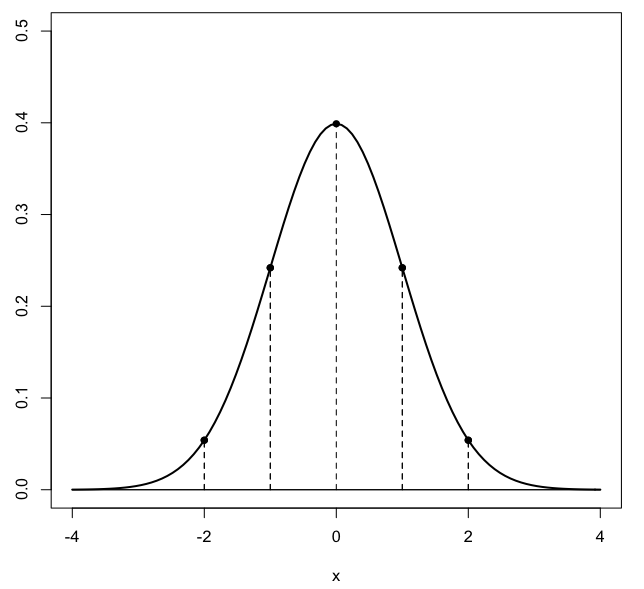
\includegraphics [scale=0.4] {gauss3.png} \end{center}

\title{Archimedes circle proof}
\date{}

\begin{document}
\maketitle
\Large

\label{sec:circle_proof}

$\circ$ \ Let $A$ be the area of the circle

$\circ$ \ Let $T$ be the area of the triangle formed with base $2 \pi r$ and height $r$ (i.e. the area of $T$ is $\pi r^2$).  

The method of proof is by finding a contradiction.  We will assume something next, and then prove that a contradiction results, so the assumption must be incorrect

$\circ$ \ Assume $A > T$.

That is, the difference $A - T$ is non-zero and positive: 
\[ A - T > 0 \]

Using the methods described \hyperref[sec:Archimedes_and_pi]{\textbf{here}}, we know that it is possible to construct an inscribed polygon whose area differs from $A$ by \emph{as little as we please}
\begin{center} 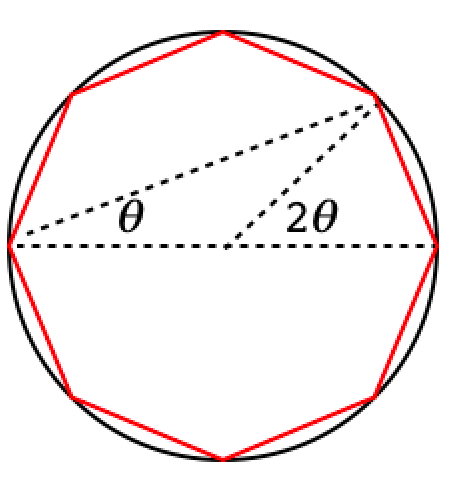
\includegraphics [scale=0.3] {piL.png} \end{center}
Here is a single sector:
\begin{center} 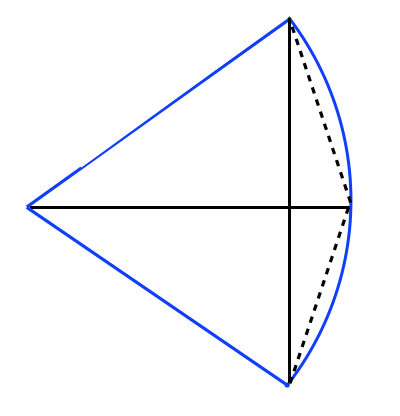
\includegraphics [scale=0.4] {inscribed_poly.png} \end{center}

In the figure, suppose that this is a sector of a blue circle, and the black vertical is one side of an inscribed polygon of $n$ sides,.

In the next step, we find a way to double the number of sides (dotted lines).  This is a simple construction, just divide the secant between two adjacent vertices, and draw the radius through that point to the edge of the circle.  By this means we can obtain a series, like $6, 12, 24, 48, 96 \dots$ sides, as Archimedes did.

Clearly, the polygon with $2n$ sides is still contained within the circle, but its area more closely approximates that of the circle.  This can be repeated forever.

Call the area of the inscribed polygon $P$.  

So what we meant by as little as we please is that $P$ can be made closer to $A$ than $T$ is, simply on the assumption that $T < A$.  Since this is an \emph{inscribed} polygon, we have
\[ A - P < A - T \]
Add $-A$ to both sides:
\[ -P < -T \]
Now, add $P + T$ to both sides:
\[ T < P \]

However, for an inscribed polygon, the area is the number of sides $n$ times the length of the base of each side, which is the perimeter, times the apothem (the vertical to the sides of the polygon), labeled $a$, times $1/2$.
\begin{center}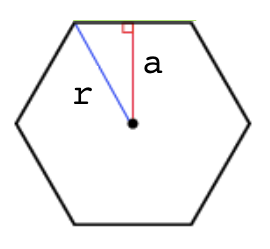
\includegraphics [scale=0.5] {apothem2.png}\end{center}

In the figure, it must be that $a < r$.  

But the perimeter is certainly less than the circumference of the circle ($2 \pi r$) so:

\[ P < \frac{1}{2} \cdot 2 \pi r \cdot r \]

By this second argument, we have shown that the area of the regular polygon, $P < T$.  However, we first showed that $T < P$.  We have reached a contradiction.  

Therefore, our assumption that $A > T$, is incorrect.  $A$ is \emph{not} greater than $T$:
\[ A \ngtr T \]

A similar argument assuming $A < T$ also leads to a contradiction.  

Since $A$ is neither greater than nor smaller than $T$ it must be equal to $T$.
\[ A = T = \frac{1}{2} \cdot 2 \pi r \cdot r  = \pi r^2 \]

The analysis is taken from Dunham's \emph{Journey Through Genius}.\

\end{document}